\documentclass[aspectratio=169,10pt]{beamer}
\usepackage[UTF8]{ctex}\usepackage{booktabs,tabularx,graphicx,amsmath,tikz}
\usetikzlibrary{arrows.meta,positioning}
\definecolor{navy}{HTML}{142B43}\definecolor{teal}{HTML}{168579}
\setbeamercolor{frametitle}{bg=navy,fg=white}\setbeamercolor{structure}{fg=teal}
\setbeamercolor{block title}{bg=teal,fg=white}\setbeamercolor{block body}{bg=teal!6}
\setbeamertemplate{navigation symbols}{}
\setbeamertemplate{footline}{\leavevmode\hbox{\begin{beamercolorbox}[wd=.80\paperwidth,ht=2.5ex,dp=1ex,leftskip=1em]{author in head/foot}青序量化研究平台\quad Project 1 / V230\end{beamercolorbox}\begin{beamercolorbox}[wd=.20\paperwidth,ht=2.5ex,dp=1ex,center]{date in head/foot}\insertframenumber/20\end{beamercolorbox}}}
\setbeamerfont{frametitle}{size=\large}\setbeamersize{text margin left=8mm,text margin right=8mm}
\begin{document}
\begin{frame}{青序量化研究平台}
\begin{block}{}课程主线保留，辅助研究有独立来源与边界\end{block}
\vspace{4mm}{\Huge\bfseries\color{navy}量化研究与证据验证}\par\vspace{4mm}
\small\begin{itemize}
\item Computational Finance · Project 1 · V230 / v2.3.0
\item 1,000只股票 · 原12经济因子 + 16个DSL公式
\item 12412408 胡博文；12410819 谢明飞；12410436 王天希
\end{itemize}
\note{各位老师、同学好。我们展示青序量化研究平台。本项目把数据、因子、含费用回测和诊断连成一个可继续维护的研究工作台。本次更新保留年度LightGBM主线，同时加入白箱因子研究、成交压力、资金归因和冻结后的观察。我们会先解释课程核心，再展示同区间实际结果，最后介绍哪些新功能已经产生证据、哪些只是接口准备。历史收益不是未来保证，语言模型建议也不是计算结果。今天所有数字来自保留的真实聚合账本，合成示例只用于软件流程。}
\end{frame}

\begin{frame}{课程要求与交付范围}
\begin{block}{}调整价格、三因子、费用账本、IC与分组仍是核心\end{block}
\small\begin{itemize}
\item 原动量/反转/低波动入口，保留12经济因子
\item 含费用回测：订单、成交、现金、持仓与独立重建
\item IC/Rank IC/五组诊断与可配置窗口
\item 扩展：28候选公式、白箱模型、压力与冻结观察
\end{itemize}
\note{我们先把课程要求理解为完整研究流程。数据必须有来源和复权规则，因子必须说明定义、方向和信息时点；回测必须把费用落实到真实模拟成交，最后用IC、分组和风险指标检查。课程至少要求三个因子，我们保留动量、反转、低波动，再维护十二个经济因子。本次新增十六个受约束公式，与原因子合成二十八个独立候选身份。报告并不只介绍新按钮，还保留原始失败、主线训练、现金账本和完整结果。材料包括报告、二十页演示、逐页讲稿及可维护源码。}
\end{frame}

\begin{frame}{平台架构}
\begin{block}{}模型更新时，复用同一套组合与成交账本\end{block}
\begin{center}\begin{tikzpicture}[node distance=3mm,every node/.style={draw=teal,fill=teal!5,rounded corners,align=center,text width=27mm,minimum height=20mm,font=\small}]
\node(a){数据快照\\字段与身份};\node(b)[right=of a]{因子与模型\\统一分数};\node(c)[right=of b]{组合与风险\\目标和现金};\node(d)[right=of c]{成交与分析\\账本与证据};
\draw[-{Stealth},teal](a)--(b);\draw[-{Stealth},teal](b)--(c);\draw[-{Stealth},teal](c)--(d);\end{tikzpicture}\end{center}
\note{平台在架构上把四件事分开。数据层处理行情、财报与交易日，因子和模型层输出股票分数，组合层把分数转成目标权重，成交层才决定实际买卖了多少。这种分离让我们可以把动量换成树模型，却不必重新实现一套现金会计。命令行、回测界面和报告都使用同一个核心。新增的策略对比与风险透镜直接读取公开日账本，因此没有原始数据的同学，也能离线复核结果。需要重新训练或按股票检查行情时，才使用本机私有快照。这样既减少了维护成本，也能明确哪些按钮是在查看证据，哪些按钮真的产生了新的实验。本次白箱路线输出同样的分数和目标权重，因此比较时共用原成交账本；严格成交压力使用另一个明确政策，原账本保留。语言模型只能提出待验证公式，不能跳过评价器直接生成可信收益。}
\end{frame}

\begin{frame}{数据来源与可见范围}
\begin{block}{}固定历史股票池，保留缺失与数据身份\end{block}
\begin{center}\small\begin{tabularx}{.97\textwidth}{lX}\toprule
项目 & 真实快照\\\midrule
资产 / 交易日 & 1,000 / 1,690\\
日频行情 / 每日估值 & 各1,656,599条\\
财务 / 历史行业区间 & 57,389 / 1,432条\\
缺失网格 & 33,401条；不伪造成交\\
\bottomrule\end{tabularx}\end{center}
\small\begin{itemize}
\item 价格：2019-10-08 至 2026-09-18
\item 固定2019年末池，不代表全部A股
\item 原始数据与Token留本地，公开聚合结果
\end{itemize}
\note{目前行情快照包含一千只股票，一百六十五万多条日线，覆盖一千六百九十个交易日。股票池在二零一九年末固定，因此不是把今天还上市的股票直接套回过去；但它也没有包括后来的新股，仍有明确的选择偏差。财报只有在公告之后才进入特征，历史行业也按有效区间匹配。我们记录缺失网格，不凭空补出可以交易的价格。原始快照和研究缓存总量约一点六三GB，新增小规模接入证据单独保存。公开仓库提供来源、哈希、聚合账本与复现方法，账号凭据和厂商原始数据不随源码发布。数据量只是基础，时点正确才决定研究能否成立。}
\end{frame}

\begin{frame}{经济因子与28个公式候选}
\begin{block}{}公式先解释，计算和筛选后才产生数值证据\end{block}
\[f_{i,t}=\frac{C_{i,t}/C_{i,t-20}-1}{s_{20}(r_i)}\]
\small\begin{itemize}
\item 12经济因子 + 16个dsl\_命名的量价公式
\item 白名单：历史滞后、滚动统计、横截面秩与安全除法
\item 不执行任意Python；所有公式用相同评价流程
\item 例：低波动Rank IC +0.072；跳月动量 −0.016
\end{itemize}
\note{原十二因子覆盖趋势、反转、风险、量价、价值、分红和盈利质量。诊断仍保留原方向：低波动的平均Rank IC约零点零七二，跳月动量约负零点零一六，不因为最后区间表现就改符号。新公式语言只允许历史滞后、滚动均值与波动、相关性、横截面秩和安全除法。例如二十日动量除以二十日波动率，是一个风险调整趋势假设。十六个新公式统一使用dsl前缀，与原经济因子区分。由此得到二十八个候选身份，避免重名覆盖原定义。IC标签属于诊断输入，不能倒流成形成日特征；重叠二十日标签也不是独立交易净值。}
\end{frame}

\begin{frame}{年度模型与严格标签边界}
\begin{block}{}此前三年训练，label\_exit严格早于形成日\end{block}
\small\begin{itemize}
\item 下一开盘进入，20交易日后开盘退出的收益秩
\item 每年更新一次：特征日与标签退出日均早于形成日
\item 主线：12标准化因子 + 12行业/市值残差
\item 辅助：训练期先选6因子，年度排名/Ridge重估
\end{itemize}
\note{模型每年更新一次，只使用形成日前三年已经可见的样本。标签从信号日的下一开盘进入，再过二十个交易日在开盘退出，因此特征日期在新年之前还不够，标签的退出日期也必须严格早于模型形成日。每日截尾、标准化和行业市值中性化都只读取当天横截面。主线LightGBM保留原参数和十二个标准化值、十二个残差值。白箱路线在二零二三之前筛定最多六个因子，此后只按年度重新估计方向或Ridge系数，alpha固定一百。二零二三到二零二四用于预选辅助策略，之后的已观察区间只能叫历史开发对照。}
\end{frame}

\begin{frame}{组合、现金与执行政策}
\begin{block}{}先形成目标，再由约束决定实际成交\end{block}
\[NAV_t=Cash_t+\sum_i u_{i,t}P^{mark}_{i,t}\]
\small\begin{itemize}
\item 原主线：50股、20日调仓、20名缓冲、允许现金
\item 最高95\%预算；单股4\%、行业25\%为形成日目标
\item 基础账本：买10bp/卖15bp；前20日成交额1\%
\item 严格压力：原股等价整手、T+1、最低佣金、税与滑点
\end{itemize}
\note{有了分数以后，先按原规则构建五十股目标，每二十日调仓，保留二十名排名缓冲。最高股票预算百分之九十五，单股目标百分之四、行业目标百分之二十五；波动预算和趋势折减都截至形成日。下一开盘成交时，涨跌停、缺价、现金不足与此前成交额上限会改变实际买卖。原账本仍按买十、卖十五个基点收费。新压力路线保持复权单位会计，用当日复权开盘价与原始开盘价的比值换算原股等价股数，整手买入，完整退出可处理零股，并限制当天新买单位出售。它确实改变成交，但没有完整模拟企业行动现金、清算或盘口。}
\end{frame}

\begin{frame}{失败记录与候选选择}
\begin{block}{}保留验证预选失败，明确后续历史重选\end{block}
\small\begin{itemize}
\item V1动量：扣费−83.57\%；零费重跑仍−75.16\%
\item V2原预选：固定最终区间+6.12\%，落后指数
\item V3先预选价值主题，随后仅+4.30\%
\item 历史复核后采用LightGBM预算版；不是独立盲测
\end{itemize}
\note{这页是策略研究最需要如实说明的部分。原始动量累计亏损百分之八十三点五七，真正把费用设成零重新运行，仍然亏损百分之七十五点一六，因此不能把失败全部归因于手续费。第二版改善了回撤，但收益没有超过指数。第三版限定八个候选，先按二零二三到二零二四年的验证结果预选价值主题，随后发现它在最终区间只赚百分之四点三。当前滚动树模型是在进一步查看历史结果后选出的。稳定仓位树模型收益更高，但验证回撤超过百分之二十五，所以没有作为默认。我们保留这些选择过程，承认最终历史区间已经参与开发，需要未来新数据验证泛化。本轮辅助路线还保留验证期预选文件；它没有因为新历史冠军而替代主线。}
\end{frame}

\begin{frame}{固定区间的收益与基准}
\begin{block}{}净收益25.13\%，最大回撤9.88\%\end{block}
\centering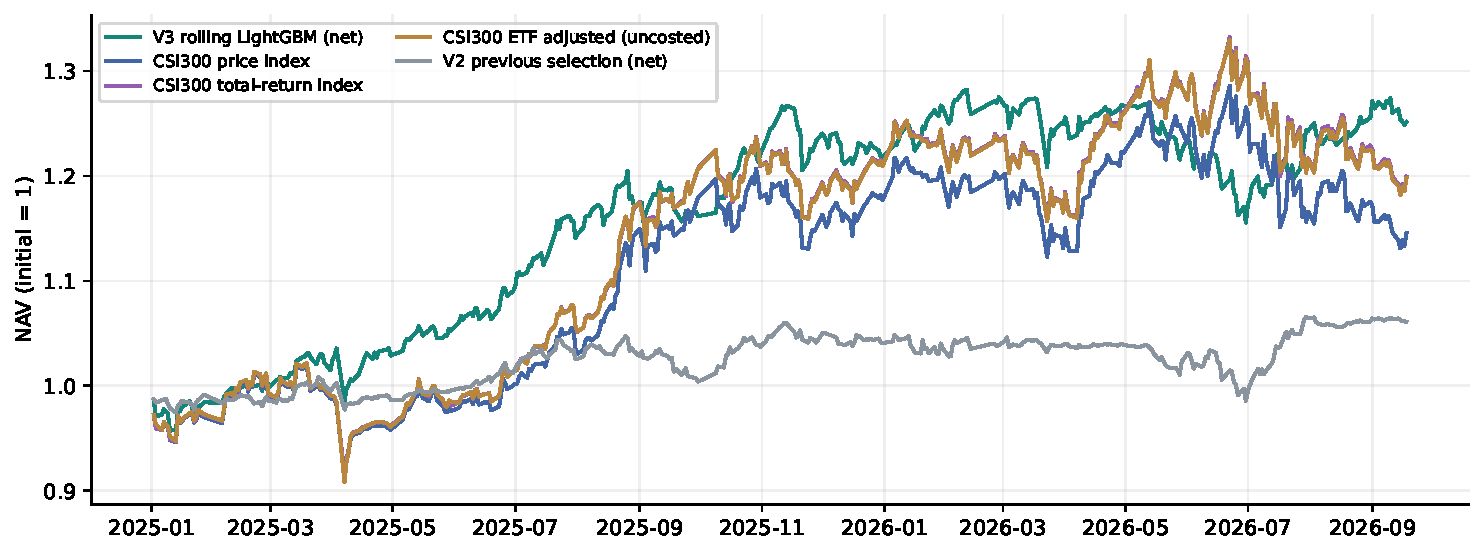
\includegraphics[width=.96\textwidth,height=.47\textheight,keepaspectratio]{figures/nav.pdf}\\[1mm]
\scriptsize\begin{itemize}
\item 价格指数14.55\%，全收益指数19.94\%
\item 分别超过10.58和5.19个百分点
\end{itemize}
\note{这张图使用二零二五年一月二日至二零二六年九月十八日相同的四百一十七个交易日。策略已经扣除实际费用，累计收益百分之二十五点一三，最大回撤百分之九点八八。沪深三百价格指数同期收益百分之十四点五五，计入红利再投资的全收益指数是百分之十九点九四。因此，策略分别超过十点五八和五点一九个百分点。这里不能把ETF代理改称全收益指数，也不能混淆百分点差和相对财富增长。为了避免首日亏损被抹掉，策略从期初资金起算，指数从前一交易日收盘起算。平台中的日期切片和策略比较采用完全相同的边界定义。}
\end{frame}

\begin{frame}{费用压力与实际成交约束}
\begin{block}{}严格情景改变费率和成交，须分别解释\end{block}
\centering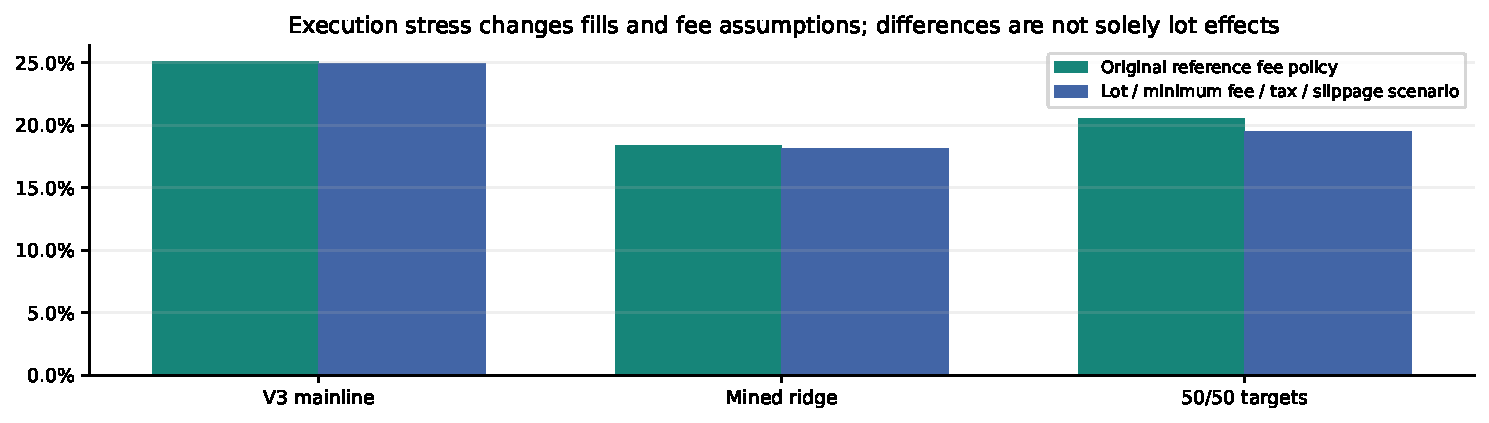
\includegraphics[width=.96\textwidth,height=.47\textheight,keepaspectratio]{figures/strict_stress.pdf}\\[1mm]
\scriptsize\begin{itemize}
\item 主线严格情景收益 24.92\%
\item 白箱Ridge 18.15\%；组合 19.49\%
\item 与基础费率不同，差额不能全归因于整手
\item 双倍基线费用、原延迟与连续运行结果保留
\end{itemize}
\note{压力测试要完整重跑成交，不能简单把成本加回净值。原主线双倍费用收益约百分之二十二点四八，延迟一天约百分之二十七点三一，这些原结果保留。新严格情景下，主线收益24.92\%，白箱Ridge为18.15\%，固定权重组合为19.49\%。严格路线另设最低佣金、买卖佣金、日期税率和滑点现金成本，所以相对原账本的收益差并不单独代表整手效应。它仍然是复权收益研究，原股等价整手和T加一约束不能被称为完整实盘结算。}
\end{frame}

\begin{frame}{白箱因子研发与模型辅助}
\begin{block}{}建议、DSL校验、实测评价各自留下来源\end{block}
\small\begin{itemize}
\item 训练期覆盖/Rank IC/冗余筛选，预算最多6因子
\item 固定白箱、排名组合、年度Ridge分别留结果
\item OpenAI兼容/Ollama接口；离线解释明确标识
\item 本次真实研究 llm\_called=false，未发生模型请求
\end{itemize}
\note{因子实验室把研究分成三个步骤。先提出可以解释的公式，经过白名单校验后计算，再按训练期覆盖、有效日期、Rank IC强度和相关性筛选，最多保留六个因子。固定经济白箱、筛选后的排名组合与年度Ridge分别回测，不能只保留一个最好结果。模型辅助层支持兼容Chat Completions的服务或本机Ollama，但本次真实研究没有发起语言模型请求，协议明确记录llm\_called为false。离线解释是确定性文本，服务返回也标为未核验建议。只有评价器重新计算得到的IC、净值和成本才进入研究证据，不能把模型说的预期收益放进成绩表。}
\end{frame}

\begin{frame}{五个候选的完整历史对照}
\begin{block}{}白箱预选保留为辅助，主线继续保留\end{block}
\centering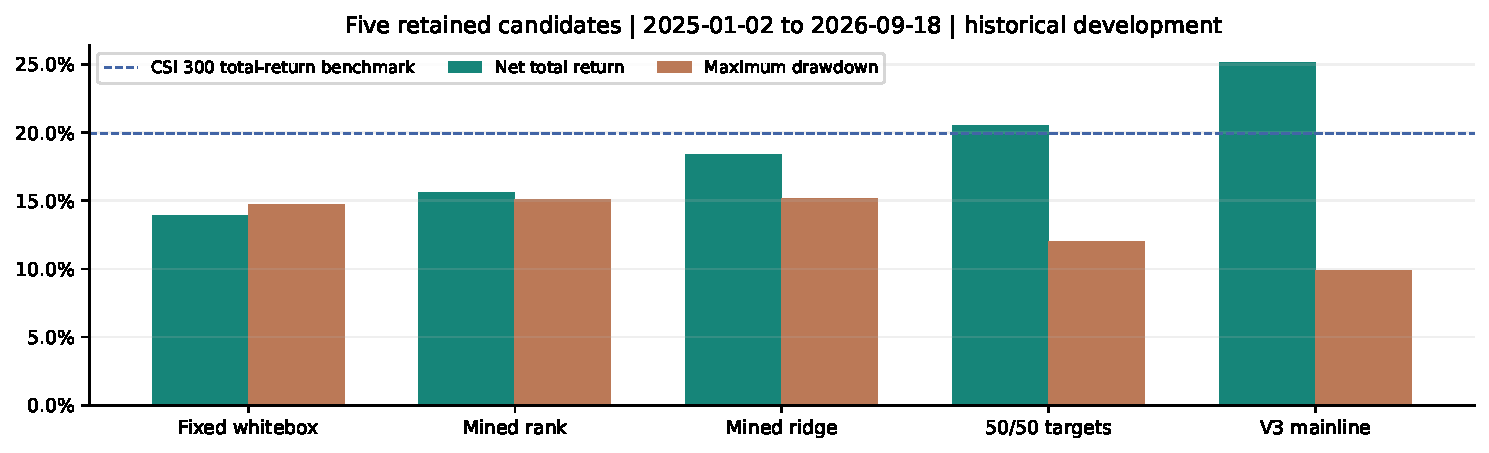
\includegraphics[width=.96\textwidth,height=.47\textheight,keepaspectratio]{figures/v4_candidates.pdf}\\[1mm]
\scriptsize\begin{itemize}
\item 2023–2024按夏普预选白箱Ridge：0.583
\item 2025起：Ridge 18.37\%；50/50组合 20.54\%
\item 主线 25.13\%；全收益指数 19.94\%
\item 全部五候选保留；历史开发对照不能改称未知盲测
\end{itemize}
\note{这页列出本轮全部五个候选，而不是只展示赢家。相同四百一十七日内，固定经济白箱收益13.90\%，筛选排名收益15.63\%，年度白箱Ridge收益18.37\%，主线与排名目标各占一半的组合收益20.54\%，主线仍为25.13\%。白箱Ridge是在二零二三到二零二四的验证夏普上预选的，但之后没有超过百分之十九点九四的全收益指数。五十对五十组合略超过全收益基准，也仍弱于主线。结论是这些方法值得继续观察，尚无证据支持替换默认策略。所有已观察结果都属于历史开发比较。}
\end{frame}

\begin{frame}{风险分析与资金账本归因}
\begin{block}{}逐股现金流加末日持仓，贡献核对组合净损益\end{block}
\[\Pi_i=S_i-B_i-C_i+V_{i,T},\qquad \sum_i\Pi_i=NAV_T-NAV_0\]
\small\begin{itemize}
\item 卖出现金流 − 买入现金流 − 实际成本 + 期末价值
\item 完全退出股票仍保留损益；成本分项有据才显示
\item 行业聚合需要明确标签；不能称因果因子归因
\item 月历、回撤恢复、滚动风险与同区间比较继续保留
\end{itemize}
\note{收益归因首先解决账本问题。每只股票的损益等于卖出现金流，减去买入现金流和实际成本，再加最后一天的持仓价值；完全退出的股票也不能被丢掉。各股损益之和应等于末日组合净值减初始资金。新账本记录佣金、税与滑点时可以分别汇总，原账本没有记录的分项保持未知。行业归因只按明确提供的标签汇总，不证明某行业或因子造成收益。已有风险透镜继续展示月收益、回撤谷底、恢复和六十日滚动统计。日期切片使用此前净值保留首日损益，未恢复回撤保持开放状态，不能把缺失日期补成已经恢复。}
\end{frame}

\begin{frame}{冻结计划与前向观察}
\begin{block}{}冻结后记录可以复查，未来表现仍待积累\end{block}
\small\begin{itemize}
\item 冻结策略/公式/系数/配置/代码/数据身份与截止日
\item 只追加截止日之后的日期；signal\_asof严格早于成交
\item 同日重试幂等；冲突、改写及链身份错误拒绝
\item 历史补录与前向纸面记录分别标识，非实盘证明
\end{itemize}
\note{当前最有价值的下一步，是先冻结规则再积累新数据。冻结文件应保留策略、公式、年度系数、训练和执行配置、代码与数据身份，以及最后已知交易日。观察只允许追加截止日之后的日期，信号形成日必须早于成交日；同样内容的重复登记返回已有记录，冲突改写被拒绝，既有记录有哈希链。冻结之前已经发生的日期，即使后来才录入，也只属于历史补录。冻结以后登记的内容首先是纸面观察；本地时钟、人工净值和哈希不能证明真实信息获取时点或账户成交。我们不把历史净值填入前向成绩，更不提前声称前向验证成功。}
\end{frame}

\begin{frame}{外部接入与尚未实测的扩展}
\begin{block}{}接口状态、原生计算和交易授权分别报告\end{block}
\small\begin{itemize}
\item Qlib 0.9.7：8表达式核对；Alpha158配置实测
\item 同花顺/SuperMind：文件桥，账号/API未连接
\item 指数增强：缺历史成分权重，尚无真实增强实测
\item 1.4.1的主要历史改动是启动修复，不能包装为策略提升
\end{itemize}
\note{外部工具接入需要区分状态。此前Qlib零点九点七在独立环境读取二十股数据，八个表达式与pandas逐项核对，还运行Alpha158的一百五十八项配置；这验证因子接口，没有训练Qlib策略，也没有替换主账本。同花顺与SuperMind提供文件桥，支持观察权重导出和模拟成交CSV核验，但账号和API未连接，没有提交订单。本次指数增强组件也保留明确门槛：没有真实历史成分权重时，不发布增强收益，不把手工样例当指数实测。历史发行一点四点一的主要用途是修复启动；启动正常、增加页面和策略优越性是不同证据，需要分别说明。}
\end{frame}

\begin{frame}{课堂演示：沿证据走一遍}
\begin{block}{}公开账本可离线查看，真实重跑依赖合法快照\end{block}
\small\begin{itemize}
\item 总览 → 主线与五候选同区间比较
\item 因子实验室 → 公式/来源/训练筛选/离线模型状态
\item 成交压力 → 资金归因 → 冻结观察的待验证状态
\item 实验档案查看订单与参数；不现场等待年度重训
\end{itemize}
\note{下面预留一分四十五秒演示。先在总览确认主线与快照截止日，打开同区间对比，说明候选使用相同日期和费用账本。在因子实验室查看公式、训练筛选来源和离线模型状态。接着查看严格政策，说明原股等价整手与复权单位仍是研究近似；打开资金归因核对损益，展示冻结计划和等待新增数据的状态。实验档案保留订单、参数和失败结果。现场用预先准备的数据；环境不可用时展示同版本PDF及证据CSV，不使用未核验截图，也不等待下载或重训。}
\end{frame}

\begin{frame}{验证、来源与复现边界}
\begin{block}{}软件核验与未来市场表现分别成立\end{block}
\small\begin{itemize}
\item 最终测试：269项通过，1项跳过；以封存日志为准
\item 界面核验：新页AppTest与独立浏览器交互通过；范围见evidence/ui\_v230
\item 主线及V4各自保存协议、输入/源码身份和核对
\item 无凭据读公开聚合结果；合法快照用于训练与逐股查询
\end{itemize}
\note{复现时先区分四件事：源码已写好，研究已产生真实输出，软件测试通过，以及界面实际完成交互。它们不能互相替代。这里列出的最终测试与界面状态都对应封存证据，检查范围以实际记录为准。独立账本从实际成交成本重建现金、单位、每日净值和收益；上游还有标签退出边界、公式前缀因果性、缺价和幂等冲突检查。公开证据支持离线查看聚合结果；真实训练及逐股行情需要合法快照。改变假设就保存新的实验身份，修正前旧结果也保留归档。工程检查不会证明未来市场一定有效。}
\end{frame}

\begin{frame}{结论：保留主线，继续积累证据}
\begin{block}{}辅助路线更可解释，仍需新数据验证\end{block}
\small\begin{itemize}
\item 主线扣费 25.13\%；历史最大回撤 9.88\%
\item 白箱/组合全部结果公开，尚不足以替代主线
\item 真实LLM服务未调用；指数增强缺权重未实测
\item 下一步：冻结规则、追加新日、同口径核验
\end{itemize}
\note{最后回到课程目标。我们保留了调整价格、明确因子、含费用成交和独立诊断，也把这些环节放进可以继续维护的工作台。主线在固定历史区间取得百分之二十五点一三净收益，但经过历史复核选择，不能说成未知盲测成功。新的白箱与组合给出了更透明的解释和另一条研究路线，完整对照尚不足以取代主线。语言模型接口没有在本轮真实调用，指数增强也没有缺权重时的假实测。下一步应冻结参数，积累真正新增的数据，并继续用相同账本、成本和基准检查。谢谢各位，欢迎针对公式、训练边界和成交记录提问。}
\end{frame}

\begin{frame}{备份：统计口径}
\begin{block}{}初始资金参与首日收益与最大回撤\end{block}
\[r_t=\frac{NAV_t}{NAV_{t-1}}-1,\qquad DD_t=1-\frac{NAV_t}{\max_{0\leq s\leq t}NAV_s}\]
\small\begin{itemize}
\item 收益：NAV终值 / 区间前收盘 − 1
\item 回撤：1 − NAV / 包含初始值的历史高点
\item 下行偏差：全部观察日作分母，目标为零
\item 月度收益复利；重叠20日标签不能连乘为净值
\end{itemize}
\note{如果老师追问统计公式，可以用这一页说明。区间第一天收益不是零，而是第一天收盘净值与前一日净值或初始资金的比值。最大回撤的高水位也包含初始资金，因此一开始就亏损不会被遗漏。年化波动采用样本标准差乘根号二百五十二，下行偏差把正收益日记为零，但分母仍然是全部观察日。月度收益由日收益复利得到，首尾不足一个月会明确显示。因子二十日远期标签存在重叠，它适合诊断排序关系，不能直接连乘当作真实投资净值。}
\end{frame}

\begin{frame}{备份：答辩问题与证据边界}
\begin{block}{}可解释、工程可用与策略有效性要分别回答\end{block}
\small\begin{itemize}
\item 为何不选新白箱？验证预选后仍未胜全收益基准
\item 模型是否参与实测？没有；离线确定性解释已标识
\item 整手/T+1是否实盘？原股等价约束，未完整企业行动结算
\item 指数增强是否已跑？缺历史真实权重，门槛尚未满足
\end{itemize}
\note{如果问新白箱是不是更好，我们回答验证预选的Ridge在后续历史只有百分之十八点三七，低于全收益基准和主线，所以继续保留辅助身份。如果问语言模型是否生成了这次成绩，回答没有，本轮协议记录未调用，所有分数和指标来自代码评价。若追问整手与T加一，说明它们限制实际模拟成交，但会计仍为复权单位，未完整处理分红现金与清算。若问指数增强，真实历史权重缺失时不会给出收益。原有负收益、预选失败和落后年份仍在档案中，冻结与新数据观察是下一步，而不是用接口准备替代验证。}
\end{frame}
\end{document}
